% by Mirella M. Moro; version: January/18/2012 @ 04:16pm
% -- 01/18/2012: more discussion on SBBD + JIDM; overall revision
% -- 09/03/2010: bib file with names for proceedings and journals; cls with shrinked {received}
% -- 08/27/2010: appendix, table example, more explanation within comments, editors' data

\documentclass[jidm,a4paper]{jidm} % NOTE: JIDM is published on A4 paper
\usepackage{graphicx,url}  % for using figures and url format
\usepackage[T1]{fontenc}   % avoids warnings such as "LaTeX Font Warning: Font shape 'OMS/cmtt/m/n' undefined"

%\usepackage{cite} % NOTE: do **not** include this package because it conflicts with jidm.bst

% Standard definitions
\newtheorem{theorem}{Theorem}[section]
\newtheorem{conjecture}[theorem]{Conjecture}
\newtheorem{corollary}[theorem]{Corollary}
\newtheorem{proposition}[theorem]{Proposition}
\newtheorem{lemma}[theorem]{Lemma}
\newdef{definition}[theorem]{Definition}
\newdef{remark}[theorem]{Remark}

% New environment definition
\newenvironment{latexcode}
{\ttfamily\vspace{0.1in}\setlength{\parindent}{18pt}}
{\vspace{0.1in}}

% ALL FIELDS UNTIL BEGIN{document} ARE MANDATORY

% The following data (volume, number and page) are given by the editors prior to publishing your article
\jidmVolume{5}
\jidmNumber{1}
\jidmYear{14}
\jidmMonth{June}
\setcounter{page}{1}


% Includes headers with simplified name of the authors and article title
\markboth{A.C. Salgado and V. Braganholo}
{JIDM - Journal of Information and Data Management}
%  -> \markboth{}{}
%         takes 2 arguments
%         ex: \markboth{M. M. Moro}{Any article title}


% Title of the article
\title{JIDM - Journal of Information \\ and Data Management\footnote{The original version of this template, which was used up to volume 3, was created by Alberto Laender and Mirella Moro}}


% List of authors
%IF THERE ARE TWO or more institutions, please use:
%\author{Name of Author1\inst{1}, Name of Author2\inst{2}, Name of Author3\inst{2}}
\author{Ana Carolina Salgado\inst{1}, Vanessa Braganholo\inst{2}}


%Affiliation and email
\institute{Universidade Federal de Pernambuco, Brazil \\ \email{acs@cin.ufpe.br}
\and Universidade Federal Fluminense, Brazil \\ \email{vanessa@ic.uff.br}
% IF THERE IS ANOTHER INSTITUTION:
%\and Name_of_the_second_institution \\
%\email{address@whatever.com}
}


% Article abstract - it should be from 100 to 300 words
\begin{abstract}
JIDM is an electronic publication focusing on information and data management in large repositories and document collections. This article introduces the journal, its scope and topics, and the submission process. Finally, it also summarizes information on SBBD, due to its close relation with the symposium.
\end{abstract}


% ACM Computing Classification System categories
\category{H.2}{Database Management}{Miscellaneous} 
\category{H.3}{Information Storage and Retrieval}{Miscellaneous}
\category{I.7}{Document and Text Processing}{Miscellaneous}

% Categories and Descriptors are available at the 1998 ACM Computing Classification System
% http://www.acm.org/about/class/1998/
%  -> \category{}{}{}
%         takes 3 arguments for the Computing Reviews Classification Scheme.
%         ex: \category{D.3.3}{Programming Languages}{Language Constructs and Features}
%                   [data types and structures]
%                   the last argument, in square brackets, is optional.

% Article keywords
\keywords{JIDM, SBBD, template}
%  -> \keywords{} (in alphabetical order \keywords{document processing, sequences,
%                      string searching, subsequences, substrings})


% THE ARTICLE BEGINS
\begin{document}

% This is optional:
\begin{bottomstuff}
% similar to \thanks
% for authors' addresses; research/grant statements
\end{bottomstuff}

\maketitle


% ARTICLE NEW SECTION
\section{Call for Contributions}

JIDM is an electronic publication focusing on information and data management in large repositories and document collections. It relates to different areas from Computer Science, including databases, information retrieval, digital libraries, knowledge discovery, data mining, geographical information systems, among others.

% ARTICLE NEW SUBSECTION
\subsection{Scope and Topics}

JIDM welcomes articles on a full range of research on information and data management, including (but not limited to):

% LIST OF ITEMS
\begin{itemize}
	\item Active Databases 
	\item Access methods and indexing 
	\item Authorization, Privacy and Security 
	\item Concurrency Control and Recovery 
	\item Data Mining and Knowledge Discovery 
	\item Data Semantics 
	\item Data Visualization 
	\item Data Warehousing 
	\item Database Design 
	\item Digital Libraries 
	\item Geographical Information Systems 
	\item Information Integration and Interoperability 
	\item Information Retrieval 
	\item Knowledge Bases 
	\item Mobile Data 
	\item Multidimensional and Temporal Databases 
	\item Multimedia Databases 
	\item Object-Orientation and Databases 
	\item Peer to peer, Parallel and Distributed Databases 
	\item Performance and Benchmarking 
	\item Query Languages and User Interfaces 
	\item Query Processing and Optimization 
	\item Scientific and Statistical Databases 
	\item Semi-structured Databases and XML 
	\item Self-managed and Autonomic Databases 
	\item Spatial Databases 
	\item Stream-based processing and Sensor Databases 
	\item Textual Databases 
	\item Web Databases 
	\item Web Services 
\end{itemize}

\subsection{Types of Submission}

JIDM welcomes \textbf{research} articles that both lay theoretical foundations and provide new insights into the aforementioned areas. JIDM also solicits \textbf{surveys} that should make a contribution to our understanding of related topics from the information and data perspective. Eventually, JIDM may publish \textbf{reports} of meetings and working groups organized to evaluate the future of a given research field. Each article will be reviewed by three different peers. 


\subsection{Submission Instructions}

Research articles should have up to \textbf{12} pages, survey articles up to \textbf{20} pages, and reports up to \textbf{6} pages. The editors should be contacted if more pages are necessary. Articles must be submitted in a PDF file according to the journal format.
Articles should be submitted by JIDM website at: 

\begin{center}
\texttt{http://seer.lcc.ufmg.br/index.php/jidm}
\end{center}



\subsection{Format Instructions}

All camera ready submissions must use LATEX. Thus, we do not provide a MS Word template. The templates for LATEX are available at the associated editor's webpage:

\begin{center}
\url{http://www.ic.uff.br/~vanessa/jidm}
\end{center}

This folder has the following files:

\begin{itemize}
	\item template.pdf
	\item jidm-template.zip
\end{itemize}

where the compacted files have: 

\begin{itemize}
	\item jidmb.bib - an example of bibliography entries
	\item jidm.cls - the latex template class for jidm
	\item jidm.bst - the latex template for bibliography entries
	\item template.tex - an example of tex file (with a figure in \textit{schedule.eps})
\end{itemize}

Prospective authors should take a look at the template.tex for more information on the format, for example: how to add more than one institution to the affiliation and  references to books \cite{Baeza-YatesR99}, book chapters \cite{BorgidaCL09}, conference papers \cite{FerreiraGALV09}, conference papers on book series (e.g., LNCS) \cite{SilvaLC96}, journal articles \cite{LaenderMNM09}, PhD thesis \cite{Moro07} and information published online\footnote{Note: in case the URL refers to a software, dataset source or any other information that does not have a proper author, it is better to include it as a footnote, e.g.: ``Biblioteca Digital Brasileira de Computa\c{c}\~{a}o: http://www.lbd.dcc.ufmg.br/bdbcomp''} \cite{xpath}. The file \textit{jidmb.bib} has examples of how to name conference proceedings and journals. In addition, Appendix A overviews the most important Latex instructions and is a ``must-read'' for authors with little or no experience in Latex, and Appendix B presents the most common errors.

\section{JIDM and SBBD}

SBBD - the Brazilian Symposium on Databases- is the official database event of the Brazilian Computer Society (SBC). It is the largest venue in Latin America for presentation and discussion of research results in the database domain. SBBD joins researchers, students and practitioners, from Brazil and abroad, for discussing problems related to the main topics in modern database technologies. 

From 2010 on, SBBD submission process is integrated with JIDM. 
Each year, SBBD has its own call for papers with specific topics and program committee. Submissions received between \textbf{December} and \textbf{May} are evaluated by SBBD PC members, while the others are evaluated by JIDM reviewers (note that there is a considerable intersection between the two sets of reviewers).

Once SBBD deadline has passed, the submissions go through a first round of revisions and the authors shall receive their reviews by middle \textbf{June}. These reviews may request the submission to be revised and the revised version must be submitted by beginning of \textbf{July} for another review round (the correct dates are published in the SBBD call for papers). The reviews and acceptances for the revised version will be sent to authors by middle \textbf{August}.


\textbf{Very important: All papers published in JIDM must have a presentation in the closest SBBD}, according to the following agenda. All papers accepted by middle August will be published in the October edition and presented at the upcoming SBBD. Papers that are accepted after that date should be published in the February JIDM edition and presented at SBBD in the following year. For example, Figure \ref{fig:schedule} illustrates the regular schedule for JIDM and SBBD, which is also represented in Table \ref{table:schedule} (in order to show how to add figures and tables to your article).


% EXAMPLE OF HOW TO INCLUDE eps FIGURES
\begin{figure}[t] % FIGURES SHOULD BE AT THE TOP [t] OR BOTTOM [b} OF PAGES
\begin{center}	% FIGURES SHOULD BE CENTERED
		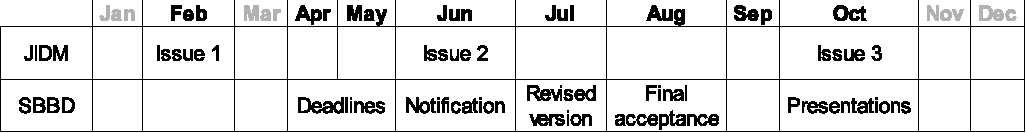
\includegraphics[width=0.9\textwidth]{schedule.pdf} % YOU MAY SHRINK YOUR FIGURE WITH width
	\caption{JIDM and SBBD schedules: as a figure\label{fig:schedule}}	
       % ALWAYS INCLUDE CAPTIONS IN YOUR FIGURES
	 % USE THE CONTENT WITHIN label FOR REFERENCING IT (USE \ref WITHIN THE TEXT)
\end{center}
\end{figure}

Papers submitted to both JIDM and SBBD must not have been simultaneously submitted to any other forum (conference or journal), nor should they have already been published elsewhere.  The acceptance of a paper implies that at least one of its authors will register for the symposium to present it. Submitted papers will be reviewed based on originality, relevance, technical soundness and clarity of presentation.

Full papers must be composed using the JIDM template. Papers exceeding the page limit of the submission type will be automatically rejected without being reviewed by the Program Committee. In addition, all papers must be submitted in PDF format. Formats other than PDF will NOT be accepted. However, exceptionally and upon request, generic postscript might be accepted.



% EXAMPLE OF HOW TO WRITE A TABLE IN LATEX
% DO CHECK http://en.wikibooks.org/wiki/LaTeX/Tables FOR MORE TIPS & TRICKS ON TABLES
\begin{table}[t]% TABLES SHOULD BE AT THE TOP [t] OR BOTTOM [b} OF PAGES
	\caption{JIDM and SBBD schedules: as a table (with different font resources)\label{table:schedule}} 
       % ALWAYS INCLUDE CAPTIONS IN YOUR TABLES
	 % USE THE CONTENT WITHIN label FOR REFERENCING IT (USE \ref WITHIN THE TEXT)

\sffamily % CHANGES THE FONT WITHIN THE TABLE TO sans serif
\begin{center} %TABLES SHOULD BE CENTERED
\begin{tabular}{r|c|c|c|c|c|c|c|c|c|c|c|c|}
	\cline{2-13}  % DRAWS HORIZONTAL LINE FROM 2nd to 13th COLUMNS
	& \rotatebox{90}{Jan } % ROTATES TEXT 90o
	& \rotatebox{90}{Feb} &\rotatebox{90}{Mar} &\rotatebox{90}{Apr} &\rotatebox{90}{May } &\rotatebox{90}{Jun} &\rotatebox{90}{Jul} &\rotatebox{90}{Aug} &\rotatebox{90}{Sep} &\rotatebox{90}{Oct} &\rotatebox{90}{Nov} &\rotatebox{90}{Dec} \\ \hline % DRAWS HORIZONTAL LINE
\multicolumn{1}{|r|}{JIDM} % THIS multicolumn JUST GUARANTEES THE VERTICAL LINE AT THE BEGINNING OF THE COLUMN
& -- & Issue 1 & -- & -- & --                         & Issue 2      & --      & --         & -- & Issue 3 & -- & -- \\ \hline
\multicolumn{1}{|r|}{SBBD} & -- &         & -- & \multicolumn{2}{|c|}{SBBD} % THIS multicolumn MERGES TWO CELLS
& Notification & Revised & Final      & -- & Presentations & -- & -- \\ 
\multicolumn{1}{|r|}{}     &    &         &    & \multicolumn{2}{|c|}{Deadlines} &              & Version & Acceptance &  &  & & \\ \hline
\end{tabular}
\end{center}
\rmfamily % RESTORES TO TIMES, SO THAT CAPTION IS WRITTEN PROPERLY
\end{table}

\section{Further Information}

Further information regarding JIDM may be found at its webpage: {\center \url{http://seer.lcc.ufmg.br/index.php/jidm} }

Other questions regarding JIDM should be emailed to the editors:

\textbf{Editor in Chief} - Ana Carolina Salgado, email: \url{jidm.eic@gmail.com}

\textbf{Associate Editor} - Vanessa Braganholo, email: \url{vanessa@ic.uff.br}

% INCLUDE BIBLIOGRAPHY WHICH MUST FOLLOW jidm.bst TEMPLATE
\bibliographystyle{jidm}
\bibliography{jidmb}
% For information on how to write bibliography entries, 
% see file jidmb.bib

%%%%%%%%%%%%%%%%%%%%%%%%%%%%%%%%%%%%%%%%%%%%%%%%%%%%%%%%%%%%%%%%%%%%%%%%%%%%%%%%%%%%%%%%%%%%%%%
\appendix
%%%%%%%%%%%%%%%%%%%%%%%%%%%%%%%%%%%%%%%%%%%%%%%%%%%%%%%%%%%%%%%%%%%%%%%%%%%%%%%%%%%%%%%%%%%%%%%
\section{LATEX Instructions}

This section overviews some basic instructions for writing an article to JIDM using LATEX.

%%%%%%%%%%%%%%%%%%%%%%%%%%%%%%%
\noindent{FIRST LINES}
%%%%%%%%%%%%%%%%%%%%%%%%%%%%%%%

The first lines of your tex file identify the document class, packages, new definitions and environments the article will use.
Specifically:

% Numbered list
\begin{enumerate}
	\item The document class must be $jidm.cls$ and is defined as follows:
	
				\begin{latexcode} 
		          $\backslash$documentclass[jidm,a4paper]\{jidm\}
		    \end{latexcode}
				
		\rmfamily Note that JIDM is published on A4 paper.

  \item You may use as many packages as you want. However, we suggest you use $graphicx$ and $url$ for figures and url format, and $fontenc$ for avoiding warnings such as ``\textit{LaTeX Font Warning: Font shape 'OMS/cmtt/m/n' undefined}''. You can define them as follows:
    
    	\begin{latexcode} 
				$\backslash$usepackage\{graphicx,url\} 
		
				$\backslash$usepackage[T1]\{fontenc\}\vspace{0.1in}
			\end{latexcode}
		
		Please note that including the package $cite$ may conflict with our template for bibliographic references ($jidm.bst$).
	
	\item You may also use new definitions, such as the ones included in JIDM template:
	
	
			\begin{latexcode} 
		  $\backslash$newtheorem\{theorem\}\{Theorem\}[section] 
		  
			$\backslash$newtheorem\{conjecture\}[theorem]\{Conjecture\}
			
			$\backslash$newtheorem\{corollary\}[theorem]\{Corollary\}
			
			$\backslash$newtheorem\{proposition\}[theorem]\{Proposition\}
			
			$\backslash$newtheorem\{lemma\}[theorem]\{Lemma\}
			
			$\backslash$newdef\{definition\}[theorem]\{Definition\}
			
			$\backslash$newdef\{remark\}[theorem]\{Remark\}
			\end{latexcode}
			
	\item You may also add new environments, such as the one included in JIDM template:

		\begin{latexcode} 
				$\backslash$newenvironment\{latexcode\} 
				
		    \{$\backslash$vspace\{0.1in\}$\backslash$setlength\{$\backslash$parindent\}\{18pt\}\} 
		    
				\{$\backslash$vspace\{0.1in\}\}
		\end{latexcode}
		 		
\end{enumerate}

%%%%%%%%%%%%%%%%%%%%%%%%%%%%%%%
\noindent{MANDATORY FIELDS}
%%%%%%%%%%%%%%%%%%%%%%%%%%%%%%%

The initial lines are followed by mandatory fields which compose the article metadata. It is very important that all of them be correctly written as follows.

\begin{enumerate}
	\item The footer of each article includes the name of the journal, and volume, number, month and year of its publication; the footer of the title page has also the initial and final page numbers; each page is also numbered (at the external margin). This information is given by the editors prior to the article publication. In order to add it to your article, use the following.
	
		\begin{latexcode} 
			$\backslash$jidmVolume\{3\}
			
			$\backslash$jidmNumber\{1\}
			
			$\backslash$jidmYear\{12\}
			
			$\backslash$jidmMonth\{February\}
			
			$\backslash$setcounter\{page\}\{3\}
		\end{latexcode}

	Note that the \textit{setcounter} establishes the number of the first page of your article.

	\item Each article has a left and right-headers composed of two parts: the abbreviated names of the authors and the title. Both parts are defined as follows:
	
		\begin{latexcode} 
			$\backslash$markboth\{A. H. F. Laender and M. M. Moro\}
			
				\{JIDM - Journal of Information and Data Management\} 
		\end{latexcode}
	
		Note that the first parameter has the authors, which are defined following these rules:
		
\begin{itemize}
	\item If there is one author, then use author's full name, such as \textit{Alberto H. F. Laender}.
	\item If there are two or three authors, then abbreviate each author's first name such as \textit{A. H. F. Laender and M. M. Moro}.
	\item If there are more than three authors, then the format is \textit{Alberto H. F. Laender et. al.}.
\end{itemize}
	
	The second parameter is the title. If the title is too long, contract it by omitting subtitles and phrases, \textit{not} by abbreviating words.
	
	\item The title of the article is defined as follows:
	
		\begin{latexcode}
				$\backslash$title\{JIDM - Journal of Information $\backslash\backslash$ and Data Management\}
		\end{latexcode}
	
		Note that if you want to break the title in two or more lines, just add a line within it with two consecutive backlashes ($\backslash\backslash$).
	
	\item After the title, you need to define the name of the authors and their affiliations, as follows.

		\begin{latexcode}
				$\backslash$author\{Alberto H. F. Laender, Mirella M. Moro\}
				
				$\backslash$institute\{Universidade Federal de Minas Gerais, Brazil $\backslash\backslash$
				
				$\backslash$email\{$\backslash$\{laender, mirella$\backslash$\}@dcc.ufmg.br\}
				
		\end{latexcode}
	
		Note that both authors belong to the same university. If you have authors from different places, you write their information as follows:
		
		\begin{latexcode}		
				$\backslash$author\{Alberto H. F. Laender$\backslash$inst\{1\}, Mirella M. Moro$\backslash$inst\{2\}\}
				
				$\backslash$institute\{Universidade Federal de Minas Gerais, Brazil $\backslash\backslash$
				
				$\backslash$email\{laender@dcc.ufmg.br\} 
				
				$\backslash$and
				
				Mirella's Own Company, Brazil $\backslash\backslash$
				
				$\backslash$email\{mirella@dcc.ufmg.br\} 	\}		 			 
		\end{latexcode}
		
	\item The next step is to add the abstract within its environment, as follows.
	
		\begin{latexcode}		
				$\backslash$begin\{abstract\}
				
Text of your abstract using from 100 to 300 words, without any references. 

Also, do avoid breaking it into paragraphs.
				
				$\backslash$end\{abstract\}
		\end{latexcode}
					
	\item After the abstract, you should include information for the ACM Computing Classification, as follows.
	
	\begin{latexcode}		
				$\backslash$category\{H.4.0\}\{Information Systems Applications\}\{General\}
	\end{latexcode}
	
	where the last argument (which contains the subject descriptors) is optional, since some categories have none. 
	Multiple subject descriptors are separated by $\backslash$\textit{and} commands, for example:  
	\begin{latexcode}
	
	$\backslash$category\{I.7.2\}\{Text Processing\}\{Document Preparation\}
	
	[Languages $\backslash$and Photocomposition])
	\end{latexcode}
	
	If you have more than one category, use a separate $\backslash$\textit{category} declaration. 
	The list of categories is available at the website \ttfamily{http://www.acm.org/about/class/1998/}. \rmfamily

	\item Then, the keywords are specified in alphabetical order as follows.
	
	\begin{latexcode}
		$\backslash$keywords\{JIDM, SBBD, template\}
	\end{latexcode}

	Note that keywords can also be expressions, such as \textit{XML query optimization}.

	\item The article then begins as follows.
	
	\begin{latexcode}
	   $\backslash$begin\{document\}
	\end{latexcode}
	
	\item It is common to thank funding agencies for research grants. If necessary, that information is defined in the \textit{bottomstuff} environment, as follows.
	
	\begin{latexcode}
		$\backslash$begin\{bottomstuff\}
	
		This work was partially funded by NSF grant number XYZ. 
	
		$\backslash$end\{bottomstuff\}	
	\end{latexcode}
	
	\item All the previous items complete the initial part of the article. Then, you need to use the \textit{$\backslash$maketitle} command, which generates and formats all the previous items, as follows.
	
		\begin{latexcode}
	   $\backslash$maketitle
	\end{latexcode}
\end{enumerate}

%%%%%%%%%%%%%%%%%%%%%%
\noindent{BODY CONTENT}
%%%%%%%%%%%%%%%%%%%%%%

The article then follows with its regular content with sections and subsections as follows.

	\begin{latexcode}
		$\backslash$section\{Section title\} \\
		\rmfamily which defines a section in first level (i.e., \textit{1. Section Title}).
	
		\ttfamily$\backslash$subsection\{Subsection title\} \\
		\rmfamily which defines a section in second level (i.e., \textit{1.1. Subsection Title}).
	
		\ttfamily$\backslash$subsubsection\{Subsubsection title\} 
		\rmfamily defines a section in third level (i.e., \textit{1.1.1. Subsubsection Title}).
	\end{latexcode}

	For further information, we refer to the following web sources:
	
	\ttfamily
\begin{itemize}
	\item http://en.wikibooks.org/wiki/LaTeX
	\item http://www.latex-project.org/
\end{itemize}
	
	\rmfamily

%%%%%%%%%%%%%%%%%%%%%%
\noindent{FINISHING YOUR ARTICLE}
%%%%%%%%%%%%%%%%%%%%%%

At the end of your article, you may add appendix sections as follows.

\begin{latexcode}
	$\backslash$appendix
	
	$\backslash$section\{Title of first appendix section\}

	Text text text
\end{latexcode}

Then, you add the dates (if you do not add these lines, the footer of the title page will be wrong), as follows:

\begin{latexcode}
	$\backslash$begin\{received\}
	$\backslash$end\{received\}
\end{latexcode}

Finally, you must refer to the bibliography style and file, as follows.

	\begin{latexcode}
		$\backslash$bibliographystyle\{jidm\}

		$\backslash$bibliography\{jidmb\}
	\end{latexcode}

\noindent where the file $jidmb.bib$ has all references. We try to keep the names of proceedings and journals following the same pattern. All references must be defined in the bib file, as follows. Please \textbf{DO NOT} include references in the tex file using \texttt{thebibliography}.

Please check that:  

\begin{itemize}
\item Words in the paper titles are capitalized;
\item Words in titles after ":" are not capitalized;
\item Conference/workshop papers have complete authors, title, proceedings name, year, paper initial and final pages, and city/country address (no series, no url, no date, no total number of pages, no publisher - see template example);
\item Conference and journal names are capitalized and are not abbreviated;
\item Journal articles must have authors, title, journal name, pages, both volume and number; 
\item Double check the template for conference papers published on Lecture Notes; 
\item Webpage can be placed as footnote instead of reference.
\item Use double "\{\{" "\}\}" in the bib file to make sure Latex will respect the capitalizations of words in titles (e.g. \texttt{title = \{\{A Query Language Based on SQL\}\}})
\item In the text, citations must not be part of the text. Instead of saying "\cite{BorgidaCL09} addresses the problem of...", please use the \texttt{citeN} command to produce sentences like this: "\citeN{BorgidaCL09} addresses the problem of..." (the latex code for this is \texttt{$\backslash$citeN\{BorgidaCL09\} addresses the problem of...}). 
\end{itemize}

\begin{latexcode}
@MISC\{xpath, \\\indent\indent
  author = \{Anders Berglund and Scott Boag and Don Chamberlin and \\\indent\indent
  Mary F. Fern$\backslash$'\{a\}ndez and Michael Kay  and Jonathan Robie and \\\indent\indent
  J$\backslash$'\{e\}r$\backslash$\^\{o\}me Sim$\backslash$'\{e\}on\},\\\indent\indent
  title = \{\{XML Path Language (XPath) 2.0, W3C Recommendation\}\},\\\indent\indent
  howpublished = \{http://www.w3.org/TR/xpath20\},\\\indent\indent
  year = \{2007\} \}\\

@INBOOK\{BorgidaCL09,\\\indent\indent
  chapter = \{\{Logical Database Design: from Conceptual to Logical Schema\}\},\\\indent\indent
  pages = \{1645-1649\},\\\indent\indent
  title = \{\{Encyclopedia of Database Systems\}\},\\\indent\indent
  publisher = \{Springer\},\\\indent\indent
  year = \{2009\},\\\indent\indent
  editor = \{Liu Ling and Tamer M. $\backslash$"\{O\}zsu\},\\\indent\indent
  author = \{Alexander Borgida and Marco A. Casanova and Alberto H. F. Laender\},\\\indent\indent
  address = \{Berlin\} \}\\

@INPROCEEDINGS\{FerreiraGALV09,\\\indent\indent
  author = \{Anderson A. Ferreira and Marcos Andr\{$\backslash$'e\} Gon$\backslash$c\{c\}alves and Jussara\\\indent\indent
	M. Almeida and Alberto H. F. Laender and Adriano Veloso\},\\\indent\indent
  title = \{\{SyGAR - A Synthetic Data Generator for Evaluating Name Disambiguation\\\indent\indent
	Methods\}\},\\\indent\indent
  booktitle = ecdl,\\\indent\indent
  year = \{2009\},\\\indent\indent
  pages = \{437-441\},\\\indent\indent
  address = \{Corfu, Greece\} \}\\

@ARTICLE\{LaenderMNM09,\\\indent\indent
  author = \{Alberto H. F. Laender and Mirella M. Moro and Cristiano Nascimento\\\indent\indent
	and Patr$\backslash$'\{$\backslash$i\}cia Martins\},\\\indent\indent
  title = \{\{An X-ray on Web-available XML Schemas\}\},\\\indent\indent
  journal = sigmodrecord,\\\indent\indent
  year = \{2009\},\\\indent\indent
  volume = \{38\},\\\indent\indent
  pages = \{37-42\},\\\indent\indent
  number = \{1\} \}\\

@PHDTHESIS\{Moro07,\\\indent\indent
  author = \{Mirella M. Moro\},\\\indent\indent
  title = \{\{The Role of Structural Aggregation for Query Processing over XML Data\}\},\\\indent\indent
  school = \{University of California, Riverside (UCR)\},\\\indent\indent
  year = \{2007\},\\\indent\indent
  address = \{USA\} \}\\

@INBOOK\{SilvaLC96,\\\indent\indent
  chapter = \{\{An Approach to Maintaining Optimized Relational Representations\\\indent\indent
	of Entity-Relationship Schemas\}\},\\\indent\indent
  pages = \{292-308\},\\\indent\indent
  title = \{Conceptual Modeling\},\\\indent\indent
  publisher = \{Springer\},\\\indent\indent
  year = \{1996\},\\\indent\indent
  editor = \{Bernhard Thalheim\},\\\indent\indent
  author = \{Altigran Soares da Silva and Alberto H. F. Laender and Marco A. Casanova\},\\\indent\indent
  volume = \{1920\},\\\indent\indent
  series = \{Lecture Notes in Computer Science\},\\\indent\indent
  booktitle = er \}
  
\end{latexcode}

%%%%%%%%%%%%%%%%%%%%5
\section{Most Common Errors}

This section lists the most common errors when writing your paper. Note that \textit{any} of these errors will certainly make the editors contact you for correction.

\begin{itemize}
	\item Files do not compile. Editors will create the pdf files from the tex sources you submitted.
	\item Refering to work as ``paper'': you should refer to your work as article.
	\item JIDM metadata different from pdf file: author names must be exactly the same in the pdf as in the metadata at JIDM website [including abbreviations and uppercase letters].
	\item Generic categories: the item ``Categories and Subject Descriptors'' should be other than ``Databases'' (since that is too generic).
	\item Wrong header: with two or three authors, the header is as ``A. H. F. Laender and M. M. Moro''; otherwise, it is ``Alberto H. F. Laender et. al.'' (use $\backslash markboth$).
	\item Acknowledgments as section/subsection: acknowledgments must be in the appropriate place (using environment $\backslash bottomstuff$).
	\item Long/wrong abstract: abstract should have only one paragraph; in the jidm metadata, it cannot have tex commands.
	\item Incomplete/wrong references: *all* references must strictly follow JIDM template, i.e., conference/workshop papers with complete authors, title, proceedings name, year, paper initial and final pages, and city/country address (no series, no url, no date, no total number of pages, no publisher - see template example); journal articles must have authors, title, journal name, pages, both volume and number; double check the template for conference papers published on Lecture Notes; webpage can be footnote instead of reference.
	\item Undefined references.
	\item Style: try to avoid orphan words (one word alone in one line), orphan lines (one line alone at the beginning of a page), single subsections (e.g., section 3, subsection 3.1, section 4); place figures and tables at the top \url{[t]} or bottom \url{[b]} of your pages.
	\item File compiles with warnings: try to eliminate all warnings, they may affect the final pdf.
	\item Wrong characters: words in Portuguese (even inside bib file) must have proper characters (e.g., Computa$\backslash$c\{c\}$\backslash$\textasciitilde\{a\}o).
	\item Outdated template: check the website for the updated template (which corrected some errors from the previous one).
\end{itemize}
	


\begin{received}
\end{received}

\end{document}
